\chapter{Generative Diffeomorphic Deformation Models}
Generative models have been successfully applied to a wide range of medical image analysis tasks such as image registration \cite{balakrishnan2019voxelmorph}, segmentation \cite{dong2017automatic} and visual feature attribution \cite{baumgartner2018visual}. Of particular interest are deformation-based models due to their ability to closely model the gradual changes occuring in biological processes.
%In contrast to the purely convolution approach, which is in essentially a universal function approximator, deformation-based models are constrained to operations that closely match the actual processes observed in human tissue.
%Particularly in the case of MRI data, voxel intensities are relative, deformation better than additional map

A deformation can be described by a diffeomorphism, a function which is differentiable and invertible, and therefore topology preserving. It follows that by using a diffeomorphic approach, a model can be limited to a set of more realistic operations which generally results in more interpretable outputs.

In this section, we discuss the general architecture of our model. We first examine the brain registration model proposed in \cite{balakrishnan2019voxelmorph} \cite{dalca2018unsupervised} followed by a discussion of our adaptations for the generative brain aging task.

\section{Diffeomorphic Image Registration}
\label{chap:voxelmorph}
In medical imaging, deformable image registration tackles the problem of warping one image onto another. More formally, given two scans $x$ and $y$, the aim is to find a deformation function $\Phi$ such that $x \circ \Phi$ is similar to $y$.

\subsection{Voxelmorph} \label{sec:vox}
Dalca et al \cite{dalca2018unsupervised} propose a deep learning architecture to learn such a mapping for 3-dimensional MRI brain data. Formally, given $x$ and $y$ the model generates a stationary velocity field $v$ which defines the deformation ${\Phi : \R^3 \rightarrow \R^3}$ mapping $x$ to $y$ through the ordinary differential equation (ODE)

\begin{equation} \label{eq:voxODE}
	\frac{\partial \Phi^{(t)}}{\partial t} = v(\Phi^{(t)})
\end{equation}

where $\Phi^{(0)} = id$ is the identity transformation and t is time.
The final deformation field $\Phi^{(1)}$ is then obtained by integrating the field $v$ over time $t = [0, 1]$, which is computed numerically using the scaling and squaring method.

In group theory, $v$ is a member of the Lie algebra and is exponentiated to produce $\Phi^{(1)} = \exp(v)$.
The collection $\{\Phi^{(t)}\}_{t \; \in \; [0,1]}$ forms a one-parameter subgroup of diffeomorphisms and therefore for any scalars $t$ and $t'$ we have 
\begin{equation} \label{eq:voxoneparamsubgroup}
	\exp((t + t')v) = \exp(tv) \circ \exp(t'v)
\end{equation}

where $\circ$ is a composition map associated with the Lie group. Consequently, we can then use the recurrence
\begin{equation} \label{eq:voxrecurrence}
	\Phi^{(1/2^{(t-1)})} = \Phi^{(1/2^{t})} \circ \Phi^{(1/2^{t})}
\end{equation}

starting from $\Phi^{(1/2^T)}$ to obtain $\Phi^{(1)} = \Phi^{(1/2)} \circ \Phi^{(1/2)}$ where $T$ is chosen such that $v \approx 0$.

The model uses a variational inference method to generate a stationary displacement field $z$ which defines the deformation $\Phi_z$ through the ODE (\ref{eq:voxODE}). The prior probabilty of $z$ is modeled as
\begin{equation}
	p(z) = \mathcal{N}(z; 0, \Sigma_z)
\end{equation}

Spatial smoothness of z is is encouraged by letting ${\Sigma_z^{-1} = \Lambda_z = \lambda L}$ where $\Lambda_z$ is a precision matrix, $L$ is the Laplacian of a neighborhood graph defined as $L = D - A$, with graph degree matrix $D$ and voxel adjacency matrix $A$, and $\lambda$ denotes a parameter controlling the scale of the velocity field.

The target image $y$ is interpreted as a noisy observation of the warped image~$x$
\begin{equation}
	p(y|z;x) = \mathcal{N}(y; x \circ \Phi_z, \sigma^2 \mathbbm{I})
\end{equation}

with $\sigma^2$ reflecting the variance of the additive noise.

A likely registration field $\Phi_z$ can then obtained by sampling $z$ from the posterior distribution $p(z | x; y)$.
However, computing this distribution is intractable in this setting and hence a variational approach is used where $z$ is sampled from an approximate posterior probability $q_\psi(z | x; y)$ parametrized by $\psi$. The distribution is modeled as a multivariate normal
\begin{equation}
	q_\psi(z | x; y) = \mathcal{N}(z; \mu_{z | x, y}, \Sigma_{z | x, y})
\end{equation}

and approximated by minimizing the KL divergence
\begin{equation}
	\begin{split}
		  &\min_\psi KL [ q_\psi(z | x; y) || p(z | x; y) ] \\
		= &\min_\psi KL [ q_\psi(z | x; y) || p(z) ] - \E_q [ \log p(y | z; x) ]
	\end{split}
\end{equation}

The complete loss function can be separated into three terms denoted as follows
\begin{equation} \label{eq:voxloss}
	\begin{split}
		\mathcal{L}(\psi; \mathbf{x}, \mathbf{y})
		& = -\E_{q}[ \log p( \mathbf{x} | \mathbf{z}; \mathbf{y} ) ]
		+ \text{KL} [ q_{\psi} ( \mathbf{z} | \mathbf{x} ; \mathbf{y} ) || p ( \mathbf{z} ) ] \\[12pt]
		& = \underbrace{
			\frac{1}{2 \sigma^2} \norm{\mathbf{y} - \mathbf{x} \circ \Phi_{z}}^{2} \vphantom{\frac{1}{2_{2_2}}}
		}_{\text{reconstruction term}} \\[6pt]
		& + \frac{1}{2} \bigg[
		\underbrace{
			tr( \lambda \mathbf{D} \Sigma_{z | x; y} - \log \abs{ \Sigma_{z | x; y} } ) \vphantom{\mu_{z | x; y}^{T}}
		}_{\text{sigma term}} +
		\underbrace{
			\mu_{z | x; y}^{T} \Lambda_{z} \mu_{z | x; y}
		}_{\text{precision term}} \bigg]
	\end{split}
\end{equation}

The first term enforces similarity between the target image $y$ and the warped source image $x \circ \Phi_z$, the second term encourages the posterior to be close to the prior $p(z)$ while the third term spatially smoothes the mean $\mu_{z | x, y}$. This effect can be shown more explicitly by rewriting the precision term as $ { \frac{\lambda}{2} \sum \sum_{j \in N(I)} ( \mu[i] - \mu[j])^{2} } $, where $N(i)$ denotes the set of neighbors of voxel $i$. Both $\sigma$ and $\lambda$ are treated as hyperparameters, respectively controlling the reconstruction penalty and the magnitude of the velocity field.

\subsubsection*{Network Architecture}
The paramaters $\mu_{z | x, y}$ and $\Sigma_{z | x, y}$ are estimated by a convolutional neural network (CNN). The architecture, which takes $x$ and $y$ as input, is based on a fully convolutional 3D UNet consisting of a convolutional layer of 16 filters followed by four downsampling layers with strides of two and three upsampling layers of 32 filters each. All convolutional layers use leaky ReLU activations with $\alpha = 0.2$ and kernels of size $3\times3\times3$. See \autoref{fig:archvox} for an illustration of the generator model.

\begin{figure}
	\centering
	\usetikzlibrary{arrows}
\usetikzlibrary{fit}

\tikzset{
	pics/conv/.style n args={5}{
		code = {
			\draw[draw=black] (#1, #2) rectangle ++ (1, 3) node[rotate=90, pos=0.5] {\large $#3 \times #4 \times #3$};
			\node[below] at (#1+0.5, #2+3.1) {\large #5};
		}
	},
	pics/text/.style n args={5}{
		code = {
			\draw[draw=black] (#1, #2) rectangle ++ (1, 3) node[rotate=#4, pos=0.5] {\huge #3};
			\node[below] at (#1+0.5, #2+3.1) {\large #5};
		}
	}
}

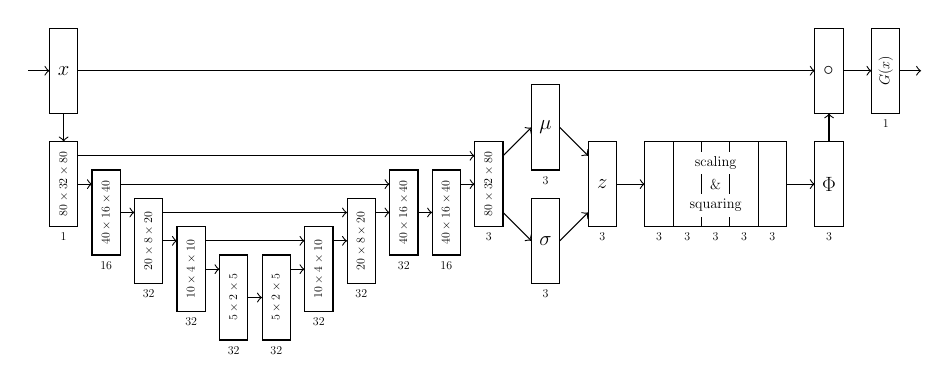
\begin{tikzpicture}[scale=0.36, line/.style={>=latex}, every node/.style={scale=0.36}, y=-1cm] 

	\pic{text={0}		{-4}	{$x$}	{0}	{}};

	\pic{conv={0}		{0}	{80}	{32}	{1}};
	\pic{conv={1.5}		{1}	{40}	{16}	{16}};
	\pic{conv={3}		{2}	{20}	{8}	{32}};
	\pic{conv={4.5}		{3}	{10}	{4}	{32}};
	\pic{conv={6}		{4}	{5}	{2}	{32}};
	\pic{conv={7.5}		{4}	{5}	{2}	{32}};
	\pic{conv={9}		{3}	{10}	{4}	{32}};
	\pic{conv={10.5}	{2}	{20}	{8}	{32}};
	\pic{conv={12}		{1}	{40}	{16}	{32}};
	\pic{conv={13.5}	{1}	{40}	{16}	{16}};
	\pic{conv={15}		{0}	{80}	{32}	{3}};
	
	\pic{text={17}		{-2}	{$\mu$}	{0}	{3}};
	\pic{text={17}		{2}	{$\sigma$}	{0}	{3}};
	
	\pic{text={19}		{0}	{$z$}	{0}	{3}};

	\pic{text={21}		{0}	{}	{0}	{3}};
	\pic{text={22}		{0}	{}	{0}	{3}};
	\pic{text={23}		{0}	{}	{0}	{3}};
	\pic{text={24}		{0}	{}	{0}	{3}};
	\pic{text={25}		{0}	{}	{0}	{3}};
	
    	\node [fill=white, inner sep=5pt] at (23.5, 0.75) {\Large scaling};
	\node [fill=white, inner sep=5pt] at (23.5, 1.5) {\Large \&};
    	\node [fill=white, inner sep=5pt] at (23.5, 2.25) {\Large squaring};

	\pic{text={27}	 	{0}	{$\Phi$}	{0}	{3}};
	
	\pic{text={27}		{-4}	{$\circ$}{90}	{}};
	
	\pic{text={29}		{-4}	{\Large $G(x)$}	{90}	{1}};

	\draw[->] (-0.75, -2.5) -- (0, -2.5);
	\draw[->] (0.5, -1) -- (0.5, 0);

	\draw[->] (1, 1.5) -- (1.5, 1.5);
	\draw[->] (2.5, 2.5) -- (3, 2.5);
	\draw[->] (4, 3.5) -- (4.5, 3.5);
	\draw[->] (5.5, 4.5) -- (6, 4.5);
	\draw[->] (7, 5.5) -- (7.5, 5.5);
	\draw[->] (8.5, 4.5) -- (9, 4.5);
	\draw[->] (10, 3.5) -- (10.5, 3.5);
	\draw[->] (11.5, 2.5) -- (12, 2.5);
	\draw[->] (13, 2.5) -- (13.5, 2.5);
	\draw[->] (14.5, 1.5) -- (15, 1.5);

	% distribution
	\draw[->] (16, 0.5) -- (17, -0.5);
	\draw[->] (16, 2.5) -- (17,  3.5);

	\draw[->] (18, -0.5) -- (19,  0.5);
	\draw[->] (18, 3.5) -- (19,  2.5);
	
	\draw[->] (20, 1.5) -- (21,  1.5);
	
	\draw[->] (26, 1.5) -- (27,  1.5);

	\draw[->] (27.5, 0) -- (27.5, -1);
	
	\draw[->] (1, -2.5) -- (27, -2.5);

	\draw[->] (28, -2.5) -- (29,  -2.5);
	\draw[->] (30, -2.5) -- (30.75, -2.5);

	% skip connections
	\draw[->] (1, 0.5) -- (15, 0.5);
	\draw[->] (2.5, 1.5) -- (12, 1.5);
	\draw[->] (4, 2.5) -- (10.5, 2.5);
	\draw[->] (5.5, 3.5) -- (9, 3.5);
	
	%\node [fill=white, inner sep=5pt] at (10.25, 2) {skip connections};

\end{tikzpicture}

	\caption{}
	\label{fig:archvox}
\end{figure}

Given $\mu_{z | x, y}$ and $\Sigma_{z | x, y}$, the subsequent layer then samples a new stationary velocity field $ { z_k \sim \mathcal{N}(\mu_{z | x, y}, \Sigma_{z | x, y}) } $ using the reparameterization trick \cite{kingma2013auto}, which is then integrated using newly introduced scaling and squaring layers to compute $\Phi_{z_k} = \exp(z_k)$. Specifically, one such layer performs a differentiable vector field composition, that is, given vector fields $a$ and $b$, it computes $(a \circ b)(p) = a(b(p))$ for each voxel $p$. Note that linear interpolation is used in $a$ as $b(p)$ generally yields a non-integer location. The recurrence in \autoref{eq:voxrecurrence} is implemented using $T = 7$ of these layers. Finally, a spatial transform layer applies the deformation field $\Phi_{z_k}$ to the source image $x$ to obtain $x \circ \Phi_{z_k}$.

The network is implemented in Keras with a Tensorflow backend and trained end-to-end using the Adam \cite{kingma2014adam} optimizer.

\section{Adaptation for Brain Aging}
While the tasks of brain registration and generative brain aging may not appear to have much in common at first, both can be described in terms of learning a deformation function. As such, the approach used in \cite{balakrishnan2019voxelmorph} can presumably be adapted to suit brain aging as well. However, while there are simililarites, a number of key differences in the problem settings require modifications to the model design.

Most importantly, the brain registration task as defined in \cite{balakrishnan2019voxelmorph} and described above is an unsupervised learning problem where both the source image $x$ and the target image $y$ are available in the prediction step. Conversely, since the goal of the brain aging task is to predict the future state of $x$, the aged target image $y$ is only available in training and therefore cannot be a part of the model's input.

Furthermore, the learned deformations for the brain aging task can be expected to be much smaller in scale and therefore, the noise introduced as part of the reconstruction term in \autoref{eq:voxloss} may have a negative effect on the model performance.

Finally, while intermediate deformations $\Phi^{(t)}$ for time steps $t \notin \{0, 1\}$ are not of primary interest in the brain registration task, the ability to predict a brain image $G(x) = x \circ \Phi_z^{(t)}$ for arbitrary $t$ promises valuable insights into the progression of neurodegenerative diseases as well as the brain's aging process in general.
Furthermore, the ability to train on image pairs over a large range of different time steps is also beneficial as the number of image pairs for any particular fixed $t$ is very limited. Moreover, training on a continuous range of time steps as opposed to a limited number of fixed intervals should result in improved generalization.

\subsection{Adversarial Loss}
% maybe say what we do first, then why?
%First, we replace the reconstruction term of the loss function \ref{eq:voxloss} with an adversarial loss.

As described above, the model input is restricted to the source image $x$ and, without access to $y$, predicting differences between the source $x$ and target $y$ that are not related to aging, such as artifacts introduced during scaning or preprocessing (e.g. skull remnants or misalignment), is virtually impossible. As a consequence, our loss function should be invariant to such changes, yet this is not the case for the reconstruction term. Moreover, the term introduces image noise which can be problematic given the small scale of aging related changes.

%As described above, the model input is restricted to the source image $x$ due to the supervised nature of the brain aging problem. However, without access to $y$, predicting differences between the source $x$ and target $y$ that are not related to aging, such as artifacts induced during scaning or preprocessing (e.g. skull remnants or misalignment), is virtually impossible. As a consequence, our loss function should be invariant to such changes. Moreover, the reconstruction loss term in \autoref{eq:voxloss} considers $y$ to be a noisy observation of $ x \circ \Phi_z $. While this works well for relatively large deformations, aging-related changes are much smaller in scale

Therefore, we opt to replace the reconstruction loss term in \autoref{eq:voxloss} with an adversarial loss component. We realize this by adding a secondary critic network to the architecture which is trained alongside the generator in an adversarial fashion. Effectively, this tranforms the model into a Generative Adversarial Network (GAN) \cite{goodfellow2014generative}.

In the adversarial setting, a generative model $G$ and a discriminative model $D$ are engaged in a minimax game, in which the generator aims to produce outputs that to the discriminator are indistinguishable from samples drawn from a real data distribution $p_{data}$. More formally, a GAN optimizes the objective
\begin{equation}
	\min_G \max_D V(G, D) = \E_{ x \sim p_{data}(x) } [ \: D (x) \: ] 
	 - \E_{ z \sim p_z(z) } [ \: 1 - D (G(z))) \: ]
\end{equation}

where $D(x)$ is a probability and $z$ is usually sampled from a latent distribution. However, in the brain aging setting the goal is to transform a source image $x$ in a way that resembles the actual aging process and therefore we get the revised objective
\begin{equation}
	\begin{split}
		\min_G \max_D V(G, D) = \; & \E_{ (x, y, t) \sim p_{data} } [ \: D (x, y, t) \: ] \\
		 - & \E_{ (x, t) \sim p_{data} } [ \: 1 - D (x, G(x), t)) \: ]
	\end{split}
\end{equation}

where the image pair $(x, y)$ and the corresponding age difference $t$ are samples from the real data distribution. Note that in order to avoid the issue of mode collapse, where the generator outputs the same image for all inputs, the discriminator also observes $x$. Furthermore, to enable the discriminator to discern pairs with differing time steps, we additionally pass $t$ as an input. Both $G$ and $D$ are implemented as neural networks which are trained in an alternating fashion. 

We use a variation of the original GAN known as Wasserstein GAN (WGAN) \cite{arjovsky2017wasserstein} in which the discriminator $D$ is replaced by a critic with real-valued outputs instead of probabilities. The critic is limited to the set of 1-Lipschitz functions, which is enforced by imposing a gradient penalty as proposed in \cite{gulrajani2017improved}.

\subsection{Additional Loss Terms}
In addition to the adversarial loss we also examine four additional loss terms and their effects on the model performance.

\subsubsection*{Age Regressor} \label{sec:adaagereg}
To encourage our model to generate realistically aged $G(x) = x \circ \Phi^{(t)} $ with respect to time step $t$, we use a pre-trained age regressor $R$ to estimate the apparent age of $G(x)$.
Let $ a_x $ denote a patient's age at the time of taking image $x$ and $ \hat a_x = A(x)$ denote the age as estimated by the age regressor on $x$. As a side note, for the generator we generally assume $t \in [0, 1]$ normalized by $\max_{(x, y) \in \mathcal{D}_{train}} a_y - a_x $, the maximum time step occuring in the training data, and therefore $t_{(x, y)} \neq a_y - a_x$ in general.

We consider two different possible loss terms 
\begin{equation}
	\begin{split}
		(1) \quad \mathcal{L}_{age}(x, y, R) & = 
		| (a_y - a_x) - (\hat a_{G(x)} - a_x) | =
		| a_y - \hat a_{G(x)} | \\[8pt]
		(2) \quad \mathcal{L}_{age}(x, y, R) & =
		| (\hat a_y - \hat a_x) - (\hat a_{G(x)} - \hat a_x) | = 
		| \hat a_y - \hat a_{G(x)} |
	\end{split}
\end{equation}

with $(1)$ using ground truth labels whenever available and $(2)$ using the regressor throughout. We hypothesize (2) to be superior due to inaccuracies of the age regressor cancelling out. This assumption is supported by our experimental results in \autoref{sec:expagereg} and consequently, we use (2) for our model.

\subsubsection*{Diagnosis Classifier}
Similar to the age regressor, we also add a loss term based on a diagnosis classifier $C$ to encourage the model to understand and distinguish between different diagnoses. Let $d_x$ denote the ground truth diagnosis label assigned to $x$ (with 0 = MCI, 1 = AD) and $\hat d_x$ denote the classifier's estimated probability of the brain in image $x$ being affected by AD. As before, we examine two possible cross entropy loss terms between ground truth labels and the estimated probabilities respectively and implement $(2)$, following the same reasoning used in selecting the age regressor loss term.

\begin{equation}
	\begin{split}
		H(p, q) & = -p \log\, q - (1 - p)\log(1 - q) \\[8pt]
		(1) \quad \mathcal{L}_{dx}(x, y, C) & = 
		H(d_y, \hat d_{G(x)}) \\[8pt]
		(2) \quad \mathcal{L}_{dx}(x, y, C) & =
		H(\hat d_y, \hat d_{G(x)}) \\[8pt]
	\end{split}
\end{equation}

In addition to its use in this loss term, the classifier also serves as our baseline for the conversion prediction experiment as described in \autoref{sec:appconvpred}.

\subsubsection*{Similarity Loss}
Similar to \cite{baumgartner2018visual} and \cite{wegmayr}, we introduce an additional loss term intended to enforce similarity and identity preservation between the original image $x$ and the warped image $ x \circ \Phi^{(t)} $ by imposing an $L_1$ loss on their difference
\begin{equation}
	\mathcal{L}_{sim}( x, G ) = \norm{ x - G(x) }_1
\end{equation}

Note that we choose not to scale the similarity loss with respect to time step $t$. This is based on the observation that while the $L_1$ difference does increase for larger $t$, as depicted in \autoref{fig:l1plots}, it does so rather slowly, indicating that the $L_1$ difference is primarily caused by differences not related to aging. As a side note, this also means that the $L_1$ metric is not very well suited to validate our generative model outputs.

\begin{figure}[h]
	\centering
	\begin{subfigure}{0.48\textwidth}
		\includegraphics[width=0.9\linewidth, trim={10 30 30 30}, clip]{images/l1_diff_plots/brains} 
		\caption{full-size}
	\end{subfigure}
	\begin{subfigure}{0.48\textwidth}
		\includegraphics[width=0.9\linewidth, trim={10 30 30 30}, clip]{images/l1_diff_plots/slice.pdf}
		\caption{cropped}
	\end{subfigure}
	 
	\caption{$L_1$ difference between image pairs $(x, y)$ from our data set for both the full-size and the cropped scans. While the difference increases with $t$, it does so rather slowly with slopes of 0.007 and 0.011 respectively.}
	%TODO(explain colors, is age when image taken)
	\label{fig:l1plots}
\end{figure}

\subsubsection*{Sparseness Loss}
Finally, we encourage sparseness of the velocity field by imposing an $L_1$ loss on its magnitude
\begin{equation}
	\mathcal{L}_{sparse}( x, G ) = \norm{\mu_z}_1
\end{equation}

Note that while this loss term acts as a regularizer, the primary motivation for sparseness is to improve the interpretability of the deformation field by discouraging displacements with very little or no effect at all.

\subsubsection*{Complete Objective}
To summarize, we obtain the complete objective for the generator as follows

\begin{equation}
	\mathcal{L}_G =
		\mathcal{L}_{ws} +
		\lambda_{1} \; \mathcal{L}_{kl} +
		\lambda_{2} \; \mathcal{L}_{age} + 
		\lambda_{3} \; \mathcal{L}_{dx} + 
		\lambda_{4} \; \mathcal{L}_{sim} + 
		\lambda_{5} \; \mathcal{L}_{sparse}
\end{equation}

where $\mathcal{L}_{ws}$ is the generator's component of the Wasserstein loss function and $\mathcal{L}_{kl}$ consists of the sigma and precision terms from \autoref{eq:voxloss}. Furthermore, we treat $ \{ \lambda_i \}_{i\;\in\;1\;..\;5}$ as hyperparameters.

\subsection{Arbitrary Time Step Training and Prediction} \label{sec:adaarbtimestep}
The scaling and squaring method as described in \autoref{chap:voxelmorph} is fixed to one specific time step $t$ determined by the model configuration as well as the training data. As mentioned above, this is not necessarily an issue in the case of image registration but highly undesirable for the brain aging task. Therefore, one of our goals is to enable training and prediction on arbitrary time steps.

One straightforward approach is to abandon the scaling and squaring method in favor of iterative composition
\begin{equation}
	\Phi^{(t)} =
	\underbrace{
		\Phi^{(1 / 2^T)} \, \circ \, \ldots \, \circ \, \Phi^{(1 / 2^T)} \vphantom{\Phi^{(1 / 2^T)}_2}
	}_{\lceil 2^T \times \: t \rceil \ \text{times}}
\end{equation}

where $2^T$ is the scaling factor and $t$ is the desired time step. Given a large enough $T$, this method can handle any positive time step with arbitrary precision, however very quickly at the cost of computional unfeasibility. Similarly, we could use a two step approach, calculating the deformation $\Phi^{(\epsilon)}$ for some time step $\epsilon$ by scaling and squaring, followed by iterative composition of $\Phi^{(\epsilon)}$. While this is much faster in practice, the choice of $\epsilon$ represents a trade-off between precision, data availability and computational viability.

In addition to the final deformation field $\Phi^{(1)}$, the recurrence also yields intermediate deformations $\{ \Phi^{(1 / 2^{t})} \}_{t \; \in \; 1 .. T} $ at no additional computational cost. For instance, the computation of a deformation field corresponding to a time step of 8 years additionally yields the deformations for (and therefore the ability to predict and train on) time steps of ${ 4, 2, 1, 0.5, \ldots }$ years. While this represents an improvement, the benefits are relatively minor as we are still limited to a small and very specific set of time steps.

However, from the properties of one-parameter subgroups in \autoref{eq:voxoneparamsubgroup} we know that any two given deformations $\Phi^{(t)}$ and $\Phi^{(t')}$ can be composed to obtain ${ \Phi^{(t + t')} = \Phi^{(t)} \circ \Phi^{(t')} }$. It follows that for any time step $t \in [0, 1)$, the corresponding deformation $\Phi^{(t)}$ can be represented as a composition of deformations from a subset $\mathcal{S}^{(t)} \subset \{ \Phi^{(1 / 2^{t})} \}_{t \; \in \; 1 .. T} $ of intermediate deformations
\begin{equation}
	\Phi^{(t)} = \underset{\Phi^{(i)} \; \in \; \mathcal{S}^{(t)}}{\bigcirc} \Phi^{(i)}
\end{equation}

In other words, $\{ \Phi^{(1 / 2^{s})} \}_{s \; \in \; 1 .. T}$ can be interpreted as a set of vectors that span the space of all deformations $\Phi^{(t)}$ for $t \in [0, 1)$, where each $\Phi^{(t)}$ is uniquely represented by a binary vector in this space. Intuitively speaking, this is analogous to how any positive integer can be expressed in $base_2$ as the sum over a set of powers of 2. The deformation is computed iteratively over all squaring step as laid out in \autoref{alg:arbtimestep}. Refer to \autoref{fig:arbtimestep} for a visual example of one such composition.

The temporal precision $\epsilon$, i.e. the smallest difference in time steps representable by the model, is determined by the number of squaring steps $T$ as well as the maximum time step $t_{max}$ used during training. Specifically, $\epsilon$ is the time step corresponding to the smallest deformation field $\Phi^{(\sfrac{1}{2^T})} = \sfrac{v}{2^T}$ and therefore $\epsilon = \sfrac{t_{max}}{2^T}$. For instance, given $t_{max} = 6$ years and $T = 7$, $\epsilon = 0.046$ years or approximately $17$ days.

In practice, the efficiency of the computation can be improved by computing only the intermediate deformations up to the largest time step required for the composition of $\Phi^{(t)}$. Furthermore, predictions for time steps $t$ beyond $t_{max}$ can be generated by dynamically increasing the number of squaring layers based on $t$.

\usetikzlibrary{arrows}
\usetikzlibrary{calc}

\begin{tikzpicture}[scale=4, line/.style={>=latex}] 
	\coordinate (p00) at (1.5, 0.3);
	\coordinate (v100) at (0.1, 0.35);
	\coordinate (p01) at ($(p00) + (v100)$);
	\coordinate (v101) at (-0.1, 0.3);
	\coordinate (p02) at ($(p01) + (v101)$);
	\coordinate (v102) at (-0.35, 0.15);
	\coordinate (p03) at ($(p02) + (v102)$);
	\coordinate (v103) at (-0.35, -0.1);
	\coordinate (p04) at ($(p03) + (v103)$);
	\coordinate (v104) at (-0.35, 0.05);
	\coordinate (p05) at ($(p04) + (v104)$);
	\coordinate (v105) at (-0.3, 0.3);
	\coordinate (p06) at ($(p05) + (v105)$);
	\coordinate (v106) at (-0.1, 0.4);
	\coordinate (p07) at ($(p06) + (v106)$);

	\node[
		opacity=0.25,
		anchor=south west, 
		inner sep=0pt
	] at (-0.2,-0.2) {\includegraphics[width=88mm]{images/mri_patch_11}}; 

	\draw[step=0.2, color=black!10] (-0.2, -0.2) grid (2, 2);
	%\draw[->, line] (-0.25, 0) -- (2.05, 0);
	%\draw[->, line] (0, -0.25) -- (0, 2.05);
	
	% v4
	\draw[->, line, color=teal, very thick, densely dotted] (p03) -- node [above right] {$\vec{v_4}(\vec x \circ \Phi^{(3s)})$} (p07);

	% v2
	\draw[->, line, color=violet, very thick, dashed] (p01) -- node [below left] {$\vec{v_2}(\vec x \circ \Phi^{(s)})$} (p03);
	\draw[->, line, color=violet, very thick, dashed] (p03) -- (p05);
	\draw[->, line, color=violet, very thick, dashed] (p05) -- (p07);

	% v1
	\draw[->, line, color=black, very thick] (p00) -- node [right=3pt, at end] {$\vec x \circ \Phi^{(s)}$}
							  node [left=2pt, midway] {$\vec{v_1}(\vec x)$}
							  node [below right, at start] {$\vec x$} (p01);
	\draw[->, line, color=black, very thick] (p01) -- node [right=6pt, at end] {$\vec x \circ \Phi^{(2s)}$} (p02);
	\draw[->, line, color=black, very thick] (p02) -- (p03);
	\draw[->, line, color=black, very thick] (p03) -- (p04);
	\draw[->, line, color=black, very thick] (p04) -- (p05);
	\draw[->, line, color=black, very thick] (p05) -- (p06);
	\draw[->, line, color=black, very thick] (p06) -- node [above right, at end] {$\vec x \circ \Phi^{(7s)} =
						((\vec x \circ \Phi^{(s)}) \circ \Phi^{(2s)}) \circ \Phi^{(4s)}$} (p07);

\end{tikzpicture}




\begin{figure}
	\centering
	\usetikzlibrary{arrows}
\usetikzlibrary{calc}

\begin{tikzpicture}[scale=4, line/.style={>=latex}] 
	\coordinate (p00) at (1.5, 0.3);
	\coordinate (v100) at (0.1, 0.35);
	\coordinate (p01) at ($(p00) + (v100)$);
	\coordinate (v101) at (-0.1, 0.3);
	\coordinate (p02) at ($(p01) + (v101)$);
	\coordinate (v102) at (-0.35, 0.15);
	\coordinate (p03) at ($(p02) + (v102)$);
	\coordinate (v103) at (-0.35, -0.1);
	\coordinate (p04) at ($(p03) + (v103)$);
	\coordinate (v104) at (-0.35, 0.05);
	\coordinate (p05) at ($(p04) + (v104)$);
	\coordinate (v105) at (-0.3, 0.3);
	\coordinate (p06) at ($(p05) + (v105)$);
	\coordinate (v106) at (-0.1, 0.4);
	\coordinate (p07) at ($(p06) + (v106)$);

	\node[
		opacity=0.25,
		anchor=south west, 
		inner sep=0pt
	] at (-0.2,-0.2) {\includegraphics[width=88mm]{images/mri_patch_11}}; 

	\draw[step=0.2, color=black!10] (-0.2, -0.2) grid (2, 2);
	%\draw[->, line] (-0.25, 0) -- (2.05, 0);
	%\draw[->, line] (0, -0.25) -- (0, 2.05);
	
	% v4
	\draw[->, line, color=teal, very thick, densely dotted] (p03) -- node [above right] {$\vec{v_4}(\vec x \circ \Phi^{(3s)})$} (p07);

	% v2
	\draw[->, line, color=violet, very thick, dashed] (p01) -- node [below left] {$\vec{v_2}(\vec x \circ \Phi^{(s)})$} (p03);
	\draw[->, line, color=violet, very thick, dashed] (p03) -- (p05);
	\draw[->, line, color=violet, very thick, dashed] (p05) -- (p07);

	% v1
	\draw[->, line, color=black, very thick] (p00) -- node [right=3pt, at end] {$\vec x \circ \Phi^{(s)}$}
							  node [left=2pt, midway] {$\vec{v_1}(\vec x)$}
							  node [below right, at start] {$\vec x$} (p01);
	\draw[->, line, color=black, very thick] (p01) -- node [right=6pt, at end] {$\vec x \circ \Phi^{(2s)}$} (p02);
	\draw[->, line, color=black, very thick] (p02) -- (p03);
	\draw[->, line, color=black, very thick] (p03) -- (p04);
	\draw[->, line, color=black, very thick] (p04) -- (p05);
	\draw[->, line, color=black, very thick] (p05) -- (p06);
	\draw[->, line, color=black, very thick] (p06) -- node [above right, at end] {$\vec x \circ \Phi^{(7s)} =
						((\vec x \circ \Phi^{(s)}) \circ \Phi^{(2s)}) \circ \Phi^{(4s)}$} (p07);

\end{tikzpicture}



	\caption{Arbitrary time step scaling and squaring with $T = 3$ squaring and $ 2^T = 8 $ atomic steps, shown for one voxel $ \vec p $. The deformation $ \Phi^{(t)} $ can be approximated at any time step $ t \in [0, 1] $ by composing a subset of intermediate deformations. Note that in practice, larger $T$ are used resulting in an exponentially higher number of atomic steps and therefore a better approximation, e.g. $T = 7$ yielding $ 2^7 = 128 $ atomic steps. We calculate the deformation for all voxels $ \vec{p} $ in parallel.} \label{fig:arbtimestep}
\end{figure}

\subsection{Network Architecture}
Based on architectures applied to similar problems such as \cite{wegmayr} and \cite{baumgartner2018visual}, we expect the brain aging problem to be a more difficult task compared to brain registration as implemented in Voxelmorph. Therefore, we significantly increase the complexity of the UNet model as shown in \autoref{fig:archour}.
%Furthermore, for computational reasons, we generate the velocity and intermediate deformation fields in half-size and upsample the final displacement to full-size before applying it to the input image $x$. Finally,
Moreover, we experiment with a low resolution time-invariant deformation component, extracted from the UNet, to capture differences that are independent of time step $t$ such as misalignments introduced during scanning or preprocessing. Separating the deformation into two components is desirable as it allows ignoring changes independent of time and therefore aging during inference on unseen data.
However, in preliminary experiments, this component appears to overpower the time-dependent deformations resulting in poor model performance and, as a consequence, is not included in our final model architecture.

\begin{figure}
	\centering
	\usetikzlibrary{arrows}
\usetikzlibrary{fit}

\tikzset{
	pics/conv/.style n args={5}{
		code = {
			\draw[draw=black] (#1, #2) rectangle ++ (1, 3) node[rotate=90, pos=0.5] {\large $#3 \times #4 \times #3$};
			\node[below] at (#1+0.5, #2+3.1) {\large #5};
		}
	},
	pics/text/.style n args={5}{
		code = {
			\draw[draw=black] (#1, #2) rectangle ++ (1, 3) node[rotate=#4, pos=0.5] {\huge #3};
			\node[below] at (#1+0.5, #2+3.1) {\large #5};
		}
	}
}

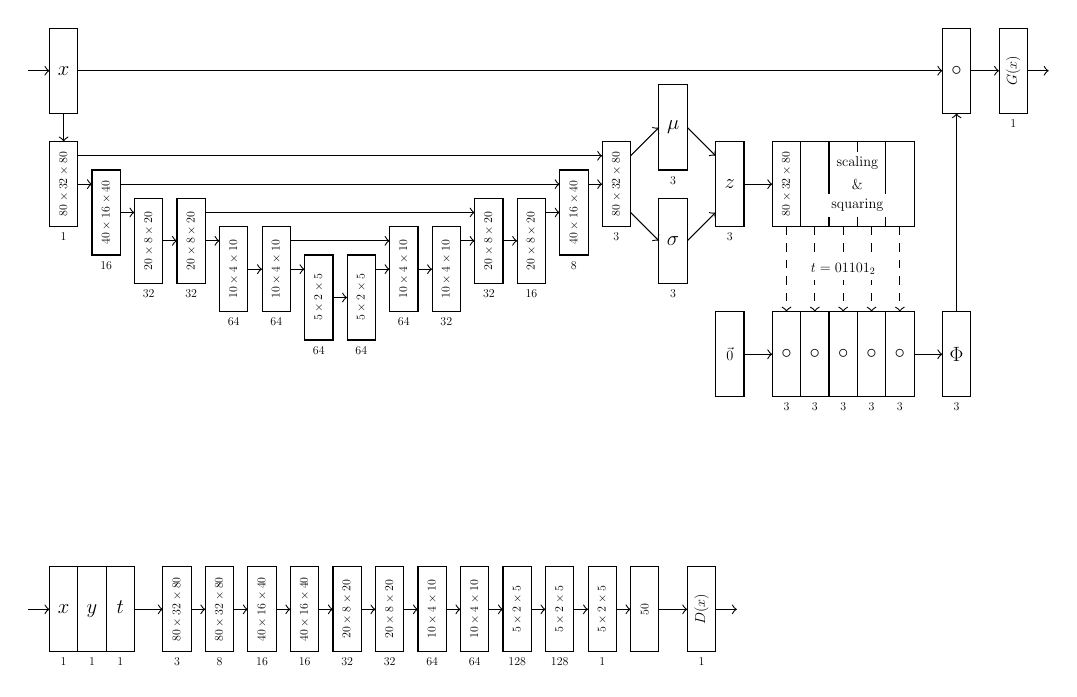
\begin{tikzpicture}[scale=0.36, line/.style={>=latex}, every node/.style={scale=0.36}, y=-1cm] 

	\pic{text={0}		{-4}	{$x$}	{0}	{}};

	\pic{conv={0}		{0}	{80}	{32}	{1}};
	\pic{conv={1.5}		{1}	{40}	{16}	{16}};
	\pic{conv={3}		{2}	{20}	{8}	{32}};
	\pic{conv={4.5}		{2}	{20}	{8}	{32}};
	\pic{conv={6}		{3}	{10}	{4}	{64}};
	\pic{conv={7.5}		{3}	{10}	{4}	{64}};
	\pic{conv={9}		{4}	{5}	{2}	{64}};
	\pic{conv={10.5}	{4}	{5}	{2}	{64}};
	\pic{conv={12}		{3}	{10}	{4}	{64}};
	\pic{conv={13.5}	{3}	{10}	{4}	{32}};
	\pic{conv={15}		{2}	{20}	{8}	{32}};
	\pic{conv={16.5}	{2}	{20}	{8}	{16}};
	\pic{conv={18}		{1}	{40}	{16}	{8}};
	\pic{conv={19.5}	{0}	{80}	{32}	{3}};
	
	\pic{text={21.5}	{-2}	{$\mu$}	{0}	{3}};
	\pic{text={21.5}	{2}	{$\sigma$}	{0}	{3}};
	
	\pic{text={23.5}	{0}	{$z$}	{0}	{3}};

	\pic{conv={25.5}	{0}	{80}	{32}	{}};
	\pic{text={26.5}	{0}	{}	{0}	{}};
	\pic{text={27.5}	{0}	{}	{0}	{}};
	\pic{text={28.5}	{0}	{}	{0}	{}};
	\pic{text={29.5}	{0}	{}	{0}	{}};
	
    	\node [fill=white, inner sep=5pt] at (28.5, 0.75) {\Large scaling};
	\node [fill=white, inner sep=5pt] at (28.5, 1.5) {\Large \&};
    	\node [fill=white, inner sep=5pt] at (28.5, 2.25) {\Large squaring};

	\pic{text={23.5}	{6}	{\Large $\vec{0}$}	{0}	{}};
	\pic{text={25.5}	{6}	{$\circ$}	{0}	{3}};
	\pic{text={26.5}	{6}	{$\circ$}	{0}	{3}};
	\pic{text={27.5}	{6}	{$\circ$}	{0}	{3}};
	\pic{text={28.5}	{6}	{$\circ$}	{0}	{3}};
	\pic{text={29.5}	{6}	{$\circ$}	{0}	{3}};
	
	\pic{text={31.5}	{6}	{$\Phi$}	{0}	{3}};
	
	\pic{text={31.5}	{-4}	{$\circ$}{0}	{}};
	
	\pic{text={33.5}	{-4}	{\Large $G(x)$}	{90}	{1}};

	\draw[->] (-0.75, -2.5) -- (0, -2.5);
	\draw[->] (0.5, -1) -- (0.5, 0);

	%\draw[->] (22.75, 7.5) -- (23.5, 7.5);
	\draw[->] (24.5, 7.5) -- (25.5, 7.5);
	
	\draw[->, dashed] (26, 3) -- (26, 6);
	\draw[->, dashed] (27, 3) -- (27, 6);
	\draw[->, dashed] (28, 3) -- (28, 6);
	\draw[->, dashed] (29, 3) -- (29, 6);
	\draw[->, dashed] (30, 3) -- (30, 6);
	
    	\node [fill=white, inner sep=5pt] at (28, 4.5) {\Large $t = 01101_2$};
	
	\draw[->] (30.5, 7.5) -- (31.5,  7.5);
	\draw[->] (32, 6) -- (32, -1);
	
	\draw[->] (1, 1.5) -- (1.5, 1.5);
	\draw[->] (2.5, 2.5) -- (3, 2.5);
	\draw[->] (4, 3.5) -- (4.5, 3.5);
	\draw[->] (5.5, 3.5) -- (6, 3.5);
	\draw[->] (7, 4.5) -- (7.5, 4.5);
	\draw[->] (8.5, 4.5) -- (9, 4.5);
	\draw[->] (10, 5.5) -- (10.5, 5.5);
	\draw[->] (11.5, 4.5) -- (12, 4.5);
	\draw[->] (13, 4.5) -- (13.5, 4.5);
	\draw[->] (14.5, 3.5) -- (15, 3.5);
	\draw[->] (16, 3.5) -- (16.5, 3.5);
	\draw[->] (17.5, 2.5) -- (18, 2.5);
	\draw[->] (19, 1.5) -- (19.5, 1.5);

	% distribution
	\draw[->] (20.5, 0.5) -- (21.5, -0.5);
	\draw[->] (20.5, 2.5) -- (21.5,  3.5);

	\draw[->] (22.5, -0.5) -- (23.5,  0.5);
	\draw[->] (22.5, 3.5) -- (23.5,  2.5);
	
	\draw[->] (24.5, 1.5) -- (25.5,  1.5);
	
	\draw[->] (1, -2.5) -- (31.5, -2.5);

	\draw[->] (32.5, -2.5) -- (33.5,  -2.5);
	\draw[->] (34.5, -2.5) -- (35.25, -2.5);

	% skip connections
	\draw[->] (1, 0.5) -- (19.5, 0.5);
	\draw[->] (2.5, 1.5) -- (18, 1.5);
	\draw[->] (5.5, 2.5) -- (15, 2.5);
	\draw[->] (8.5, 3.5) -- (12, 3.5);
	
	%\node [fill=white, inner sep=5pt] at (10.25, 2) {skip connections};

	% --- critic ---
	\pic{text={0}		{15}	{$x\vphantom{xyt}$}	{0}	{1}};
	\pic{text={1}		{15}	{$y\vphantom{xyt}$}	{0}	{1}};
	\pic{text={2}		{15}	{$t\vphantom{xyt}$}	{0}	{1}};

	\pic{conv={4}		{15}	{80}	{32}	{3}};
	\pic{conv={5.5}		{15}	{80}	{32}	{8}};
	\pic{conv={7.0}		{15}	{40}	{16}	{16}};
	\pic{conv={8.5}		{15}	{40}	{16}	{16}};
	\pic{conv={10.0}	{15}	{20}	{8}	{32}};
	\pic{conv={11.5}	{15}	{20}	{8}	{32}};
	\pic{conv={13.0}	{15}	{10}	{4}	{64}};
	\pic{conv={14.5}	{15}	{10}	{4}	{64}};
	\pic{conv={16}		{15}	{5}	{2}	{128}};
	\pic{conv={17.5}	{15}	{5}	{2}	{128}};
	
	\pic{conv={19}		{15}	{5}	{2}	{1}};
	
	\pic{text={20.5}	{15}	{\large $50$}	{90} {}};
	\pic{text={22.5}	{15}	{\Large $D(x)$}	{90} {1}};

	\draw[->] (-0.75, 16.5) -- (0, 16.5);
	\draw[->] (3, 16.5) -- (4, 16.5);

	\draw[->] (5, 16.5) -- (5.5, 16.5);
	\draw[->] (6.5, 16.5) -- (7, 16.5);
	\draw[->] (8, 16.5) -- (8.5, 16.5);
	\draw[->] (9.5, 16.5) -- (10, 16.5);
	\draw[->] (11, 16.5) -- (11.5, 16.5);
	\draw[->] (12.5, 16.5) -- (13, 16.5);
	\draw[->] (14, 16.5) -- (14.5, 16.5);
	\draw[->] (15.5, 16.5) -- (16, 16.5);
	\draw[->] (17, 16.5) -- (17.5, 16.5);
	\draw[->] (18.5, 16.5) -- (19, 16.5);
	\draw[->] (20, 16.5) -- (20.5, 16.5);
	
	\draw[->] (21.5, 16.5) -- (22.5, 16.5);
	\draw[->] (23.5, 16.5) -- (24.25, 16.5);


\end{tikzpicture}

\vspace{30pt}

	\caption{Overview of our generator and critic network architectures. Note that the convolutional layers in the generator use batch normalization while those in the critic do not. Depending on the step of the GAN training procedure, the critic input $y$ is either a real or a generated image.}
	\label{fig:archour}
\end{figure}

\chapter{Applications}
Our primary goal is to design a generative model $G$ capable of learning and simulating the aging process of the brain. Given an input image $x$, we can then use the trained model $G$ to generate a predicted future state of the brain $\hat y^{(t)} = G(x) = x \circ \Phi^{(t)}$ for any time step $t$.

Being able to generate realistic predictions might be beneficial in the early detection of Alzheimer's onset, in particular since existing diagnostic tools can be directly applied to predicted $\hat y$ without any necessary adaptations. Furthermore, the resulting deformation fields may yield insights into the progression and specific changes of neurodegenerative diseases.

\section{Conversion Prediction} \label{sec:appconvpred}
Early prediction of Alzheimer's Disease onset is an important area of Alz-heimer's research, with one particular interest being the Mild Cognitive Impairment (MCI) conversion problem. Given data about a patient diagnosed with MCI at some visit $v_i$, our goal is to predict the probabilty of that patient's diagnosis converting to AD over a given period of time $ \Delta $. 
In this context, we distinguish between progressive cases (pMCI) for which the diagnosis converts within $\Delta$, and stable cases (sMCI) for which it does not.

More specifically, a case is considered \textit{progressive} if there exists a pair of visits $(v_a, v_b)$ at times $(t_a, t_b)$ with $ t_b - t_a \geq \Delta $ and diagnoses $d_a = \text{MCI} $ and $d_b = \text{AD} $. Moreover, we require that the diagnosis does not revert after $v_b$, that is $ d_i = \text{AD} $ for all visits $v_i$ with $t_i > t_b$.

Conversely, a case is considered \textit{stable} if its diagnosis does not change across the entire data set and its visits span a time frame of at least $\Delta$, that is $ d_i = \text{MCI} $ for all visits $v_i$ and $ { \max_{t} t -  \min_{t} t \geq \Delta } $.

Using our model, we can generate $\hat y^{(\Delta)} = x \circ \Phi^{(\Delta)}$ and use this prediction to estimate the probability of a conversion occuring.

\section{Long-Term Prediction}
Another interesting application is to generate predictions for very large time steps. While we don't expect the model's predictions to be particulary accurate for time steps $t \gg 1$, i.e. time steps significantly exceeding the maximum time step occuring in training data, long-term predictions can be helpful in highlighting areas of significant change as well as in visualizing how the aging process of a healthy brain differs from that of a brain affected by AD.

\section{Feature Attribution}
Finally, similar to \cite{baumgartner2018visual}, our generator has the potential to feature attribution, that is, highlighting 

By training the model on different subsets of our data such as only AD or HC cases, we can 

Moreover, our model is probabilistic which allows us to produce multiple different predictions for the same input image $x$.
probabilistic model (sampling from distribution)
predict multiple images instead of just one
get heat map of changes

\chapter{Data}

\section{Synthetic Data} \label{sec:synth}
In order to validate our architecture, we first train and evaluate our model on a synthetic data set designed to yield easily interpretable results while still being similar in structure to the preprocessed brain data. TODO ref to figure with toy data

Each sample consists of a pair $(x_i, y_i)$ of $ 80 \times 96 \times 80 $ images, containing a spherical shell with a value of $-1$ on its shell and $1$ in its interior. We randomize both the sphere's radius and position within the image, and sample $t_i \sim \mathcal{U}(0, 1)$, the time step between $x_i$ and $y_i$. The shell's thickness decreases from $x_i$ to $y_i$, where the thickness in $y_i$ is defined as $d_{y_i} = (1-t) d_x$, with $d_x$ identical for all $x_i$. We explore two different backgrounds, a constant value of 0 as well as smoothed gaussian noise identical for $x_i$ and $y_i$.

We generate a total of 10'000 samples, using 60\% of the data set for training and 20\% for validation and testing each.

\section{MRI Data}
To train and validate our brain aging models, we use T1-weighted 3D MRI brain scans. We obtain a large data set of raw images with corresponding subject and image meta data from publically available sources and apply a preprocessing pipeline in order to extract, align and segment the brain tissue. Finally, we generate multiple different data sets tailored to our specific experiments.

\subsection{Data Sources}
We use a data set consisting of 19'480 brain MRI scans obtained from the publicly available Alzheimer's Disease Neuroimaging Initiative (ADNI) \cite{jack2008alzheimer} and Australian Imaging Biomarkers and Lifestyle (AIBL) \cite{ellis2009australian} studies. The study data was collected on a total of 9976 visits over a time period of 15 years involving 2794 subjects.

The dimensions of the raw scans depend on the type and model of scanner used and therefore vary slightly, with a median of $ 240 \times 256 \times 170 $. Furthermore, depending on a subject's study group assignment, images are taken at a field strengths of 1.5T or 3T.

\subsection{Image Data Preprocessing}
Our data processing pipeline consists of three primary steps:

\begin{itemize}
\item Registration
\item Extraction
\item Segmentation
\end{itemize}

Firstly, in the registration step we align the raw images to a common reference atlas using linear transformations with 12 degrees of freedom. Secondly, we extract the brain from from the surrounding non-brain tissue in what is known as skull stripping or alternatively brain extraction. Both steps are performed utilizing the FSL toolkit \cite{jenkinson2012fsl}, using the \texttt{flirt} \cite{jenkinson2001global} \cite{jenkinson2002improved} and \texttt{bet} \cite{smith2002fast} \cite{jenkinson2005bet2} commands respectively. Thirdly, we segment each voxel into one of three classes, White Matter (WM), Gray Matter (GM) and Cerebrospinal Fluid (CSF) while simultaneously correcting a scanner-related image artifact known as the bias field using FSL's \texttt{fast} \cite{zhang2001segmentation} command. The results of this operation are three voxel-wise probability maps for the different classes and we then proceed to subtract the WM map from the GM map while dropping the CSM map. This results in a new image with a number of potentially benefitial properties, where all voxel values are restricted to the range [-1, 1] and can be directly compared across different images. Note that the MR imaging process captures relative intensity differences and as a consequence, direct comparison of absolute values is in general not possible for raw or even unit gaussian normalized data. Furthermore, the operation enhances the structural contrast and removes low level variance in the image. We choose this apprach based on the assumption, that most of the information relevant to the brain aging process is contained in the structural changes of the segmentation (TODO experiment on data), with smaller differences in intensity most likely representing noise. \autoref{fig:preproc} shows the entire preprocessing pipeline and all its intermediate steps applied to one sample from our data set.

\begin{figure}
	\noindent\makebox[1.1\textwidth]{
		\centering
		\begin{tikzpicture}
	\node[inner sep=0pt, anchor=north west] (raw) at ( 0.0, 0)
		{\includegraphics[height=.4\textwidth, trim={18 0 0 0}, clip]{images/preproc/raw.pdf}};
	\node[inner sep=0pt, anchor=north east] (fov) at (16.0, 0)
		{\includegraphics[height=.4\textwidth, trim={60 0 68 0}, clip]{images/preproc/fov.pdf}};
	
	\node[inner sep=0pt, anchor=north east] (fli) at (16.0, -5.75)
		{\includegraphics[height=.4\textwidth, trim={75 0 75 0}, clip]{images/preproc/fli.pdf}};
	\node[inner sep=0pt, anchor=north west] (msk) at ( 5.5, -5.75)
		{\includegraphics[height=.4\textwidth, trim={75 0 80 0}, clip]{images/preproc/msk.pdf}};
	\node[inner sep=0pt, anchor=north west] (bet) at ( 0.0, -5.75)
		{\includegraphics[height=.4\textwidth, trim={75 0 75 0}, clip]{images/preproc/bet.pdf}};

	\node[inner sep=0pt, anchor=north east] (pv1) at (16.0, -12)
		{\includegraphics[height=.4\textwidth, trim={75 -10 75 10}, clip]{images/preproc/pve_1.pdf}};
	\node[inner sep=0pt, anchor=north west] (pv2) at ( 5.5, -12)
		{\includegraphics[height=.4\textwidth, trim={75 -10 75 10}, clip]{images/preproc/pve_2.pdf}};
	\node[inner sep=0pt, anchor=north west] (res) at ( 0.0, -12)
		{\includegraphics[height=.4\textwidth, trim={75 -10 75 10}, clip]{images/preproc/res.pdf}};
	
	\node[inner sep=0pt, anchor=north]      (sub) at (10.85, -17.75)
		{\includegraphics[height=.4\textwidth, trim={75 0 75 10}, clip]{images/preproc/sub.pdf}};

	\draw[->, very thick] (raw) -- node[below=5pt]{\texttt{robustfov}} (fov);
	\draw[->, very thick] (fov) -- node[right=10pt]{\texttt{flirt}} (fli);
	\draw[->, very thick] (fli) -- node[above=10pt, right=0pt, rotate=90]{\texttt{mask}} (msk);
	\draw[->, very thick] (msk) -- node[above=10pt, right=0pt, rotate=90]{\texttt{bet}}(bet);
	\draw[->, very thick] (bet.south) -- (pv1.north);
	\draw[->, very thick] (bet.south) -- (pv2.north);
	\draw[->, very thick] (bet.south) -- node[left=10pt]{\texttt{fast}} (res.north);
	\draw[->, very thick] (pv1) -- node[left=10pt]{\texttt{subtract}} (sub);
	\draw[->, very thick] (pv2) -- (sub);


\end{tikzpicture}

	}
	\caption{Preprocessing pipeline visualized for one sample}
	\label{fig:preproc}
\end{figure}

Note that since the primary output of our preprocessing pipeline is based entirely on segmentation masks, one could combine the T1-weighted scans with data from different brain imaging modalities such as T2-weighted MRI data or proton density (PD) scans, therefore drastically increasing the number of possible data sources. However, we do not validate or pursue this idea in the context of this thesis.

For computational reasons, we also perform downsampling with a factor of 0.5 followed by cropping to keep only the center 32 coronal slices, resulting in a final shape of $ 80 \times 32 \times 80 $. However, note that our architecture uses 3D convolutions throughout and therefore can be trained on the full-size data if desired, albeit at a significant computational penalty.

\subsection{Data Splitting} \label{sec:dat}
In order to run our experiments, we generate a number of data sets for the different settings. For the sake of notational brevity and conciseness, let $s$ denote one subject in our data set and let $v^s_i$ denote the $i$-th visit of subject s, with $V(s)$ denoting the temporally ordered set of visits $v^s_i \in V(s)$ of subject $s$, for $i \in 1 \ ..\ |V(s)|$. To improve readability, we generally omit $s$ unless required. For redundancy, MRI scans are usually performed twice resulting in two separate but very similar images for the same visit. Moreover, images taken at different magnetic field strength levels are available for some subjects. As a consequence, a visit $v_i$ typically consists of multiple images $x_{i, k} \in I(v_i)$ along with the corresponding image meta data. Finally, the examdate $t_i$ and the subject age $a_i$ at time $t_i$ as well as the diagnosis $d_i$ are available for most visits.

Our data sets are divided into five equal splits $ \{ \mathcal{S}_i \}_{i\ \in\ 0\;..\;4} $ of 20\% each which are used in various different configurations detailed in the corresponding experiment's section. We perform this split on a subject basis and do so globally, in the sense that if a subject appears in a specific data set, it is always assigned to the same split. In other words, for any pair of splits $ \mathcal{S}_i^A $ and $ \mathcal{S}_j^B $ taken from data sets $A$ and $B$ with $ i \neq j $, the intersection $ { \mathcal{S}_i^A \cap \mathcal{S}_j^B = \varnothing } $ is guaranteed to be empty.

\subsubsection*{Base Image Set} \label{sec:datsingles}
The \textit{Base Image Set} forms the foundation for all other data sets. It consists of all images $x_{i, k}$ and the meta data for the corresponding visits $v_i$ for which $t_i$ and $a_i$ are obtainable. The primary use for this set is in the training of our age regressor models.

\begin{table}[h]
	\begin{center}
		\begin{tabular}{c c c c c c c c c c c}
			\toprule
			\multirow{2}{*}{\bfseries Split} & 
			\multirow{2}{*}{\bfseries N} & 
			\multirow{2}{*}{\bfseries S} & 
			\multicolumn{2}{c}{\bfseries HC} & 
			\multicolumn{2}{c}{\bfseries MCI} & 
			\multicolumn{2}{c}{\bfseries AD} &
			\multicolumn{2}{c}{\bfseries Age} \\
			\cmidrule(lr){4-5}
			\cmidrule(lr){6-7}
			\cmidrule(lr){8-9}
			\cmidrule(lr){10-11} 
			& & & N & S & N & S & N & S & mean & std \\ 
			%------
			\cmidrule(lr){1-11}
			$\mathcal{S}_0$ &  2944 &  503 & 1286 &  274 &  961 &  172 &  697 & 137 & 75.1 & 7.4 \\
			$\mathcal{S}_1$ &  2905 &  504 & 1198 &  266 & 1018 &  181 &  689 & 139 & 75.6 & 7.2 \\
			$\mathcal{S}_2$ &  3202 &  506 & 1435 &  269 & 1036 &  178 &  731 & 132 & 76.3 & 7.4 \\
			$\mathcal{S}_3$ &  3294 &  504 & 1563 &  256 & 1025 &  192 &  706 & 136 & 75.6 & 7.4 \\
			$\mathcal{S}_4$ &  2947 &  506 & 1242 &  264 &  992 &  189 &  713 & 147 & 75.1 & 7.6 \\
			test            &  4188 &  271 &  174 &   14 & 3184 &  271 &  830 &  98 & 75.2 & 7.1 \\
			\cmidrule(lr){1-11}
			All             & 19480 & 2794 & 6898 & 1343 & 8216 & 1183 & 4366 & 789 & 75.5 & 7.4 \\
			\bottomrule
		\end{tabular}
		\caption{Overview of the base image set. $N$ refers to the number of separate images and $S$ to the number of distinct subjects. Note that for any split, the sum of subjects over all diagnoses generally exceeds the total number of subjects, since one subject may have images with different diagnoses.}
		\label{tab:baseset}
	\end{center}
\end{table}

\subsubsection*{MCI/AD Set} \label{sec:datmciad}
The \textit{MCI/AD Set} consists of the images of all visits $v^s_i$ for which the diagnosis $d^s_i \in \{MCI, AD\}$ and we have high confidence in the label, defined as follows:

We consider a visit $v^s_i$ \textit{firmly MCI} if $d^s_i$ as well as both the diagnoses of the previous and following visit $d^s_{i-1}$ and $d^s_{i+1}$ are $MCI$. Implicitly, this also means that we only consider subjects with at least three visits.

Conversely, for a visit $v^s_i$ to be considered \textit{firmly AD}, we require that both $d^s_i$ and $d^s_{i-1}$, the current and previous diagnoses, are $AD$.

Note that following these definitions, it is possible for one subject to have visits in both the MCI \textit{and} AD group, see \autoref{fig:mciad} for an illustrated example. An overview of the data set is shown in \autoref{tab:mciadset}.

\begin{figure}[h]
	\centering
	\usetikzlibrary{arrows}
\usetikzlibrary{calc}

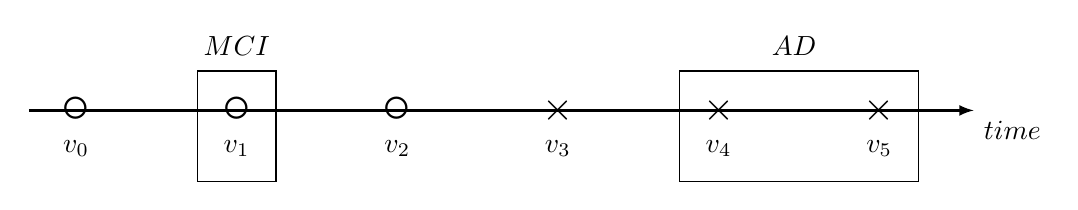
\begin{tikzpicture}[scale=1, line/.style={>=latex}] 

	\coordinate (t0) at (0, 0);
	\coordinate (t1) at (12, 0);
	\coordinate (dummy) at (0, 4);

	\draw[->, line, color=black, thick]
		(t0) --
			node [pos=0.05, below=-8.5pt] {\huge $\circ$}
			node [pos=0.05, below=7pt] {$v_0$}
			node [pos=0.22, below=-8.5pt] {\huge $\circ$}
			node [pos=0.22, below=7pt] {$v_1$}
			node [pos=0.22, above=16pt] {$MCI$}
			node [pos=0.39, below=-8.5pt] {\huge $\circ$}
			node [pos=0.39, below=7pt] {$v_2$}
			node [pos=0.56] {\Large $\times$}
			node [pos=0.56, below=7pt] {$v_3$}
			node [pos=0.73] {\Large $\times$}
			node [pos=0.73, below=7pt] {$v_4$}
			node [pos=0.81, above=16pt] {$AD$}
			node [pos=0.90] {\Large $\times$}
			node [pos=0.90, below=7pt] {$v_5$}
			node [at end, below right] {$time$}
		(t1);

	\draw[draw=black] (2.14,0.5) rectangle ++ (1,-1.4);
	\draw[draw=black] (8.26,0.5) rectangle ++ (3.04,-1.4);
	
	%\draw[->, line, color=black, very thick] (t0) -- node [at end] {$\circ$} (dummy);

\end{tikzpicture}



	\caption{Illustation of MCI and AD visits, \Large$\circ$\normalsize\;= MCI, $\times$ = AD}
	\label{fig:mciad}
\end{figure}

\vspace{20pt}

\begin{table}[h]
	\begin{center}
		\begin{tabular}{c c c c c c c c c c c}
			\toprule
			\multirow{2}{*}{\bfseries Split} & 
			\multirow{2}{*}{\bfseries N} & 
			\multirow{2}{*}{\bfseries S} & 
			\multicolumn{2}{c}{\bfseries MCI} & 
			\multicolumn{2}{c}{\bfseries AD} & 
			\multicolumn{2}{c}{\bfseries MCI $\cap$ AD} &
			\multicolumn{2}{c}{\bfseries Age} \\
			\cmidrule(lr){4-5}
			\cmidrule(lr){6-7}
			\cmidrule(lr){8-9}
			\cmidrule(lr){10-11} 
			& & & N & S & N & S & N & S & mean & std \\ 
			%------
			\cmidrule(lr){1-11}
			$\mathcal{S}_0$ &  787 & 148 &  391 &  82 &  396 &  71 &  40 &  5 & 74.4 & 7.6 \\
			$\mathcal{S}_1$ &  814 & 148 &  408 &  85 &  406 &  71 &  71 &  8 & 76.4 & 7.9 \\
			$\mathcal{S}_2$ &  909 & 150 &  451 &  82 &  458 &  72 &  45 &  4 & 77.0 & 7.9 \\
			$\mathcal{S}_3$ &  845 & 148 &  426 &  83 &  419 &  71 &  75 &  6 & 76.0 & 7.9 \\
			$\mathcal{S}_4$ &  767 & 150 &  372 &  89 &  395 &  72 &  90 & 11 & 74.9 & 8.0 \\
			\cmidrule(lr){1-11}
			All             & 4122 & 744 & 2048 & 421 & 2047 & 357 & 321 & 34 & 75.8 & 7.9 \\
			\bottomrule
		\end{tabular}
		\caption{Overview of the MCI/AD data set. $N$ refers to the number of separate images and $S$ to the number of distinct subjects. For MCI $\cap$ AD, $N$ refers to the number of images from subjects for which we have images in both groups.}
		\label{tab:mciadset}
	\end{center}
\end{table}

\subsubsection*{Image Pairs Set} \label{sec:datpairs}
The \textit{Image Pairs Set} consists of pairs of images $(x_i, x_j)$ of subject $s$ at two different visits $v_i$ and $v_j$. Of particular importance is the time step $t_j - t_i$ between $v_i$ and $v_j$. We limit the maximum time step to 6 years for computational reasons explained in \autoref{sec:adaarbtimestep}. As visualized in \autoref{fig:timestephist}, the data set is biased towards smaller $t$ with median of $1.53$, mean of $2.00$ and a standard deviation of $1.47$. To mitigate this, we calculate sample weights $w = {(| t - \bar t | + 1)}^{\sfrac{1}{2}}$, where $\bar t$ is the mean over all $t$. The resulting distribution is shown in \autoref{fig:timestephist}.

\begin{table}
	\begin{center}
		\begin{tabular}{l c c | c c c c c c}
			\toprule
			& 
			\multicolumn{2}{c}{All} &
			\multicolumn{2}{c}{\bfseries HC} & 
			\multicolumn{2}{c}{\bfseries MCI} & 
			\multicolumn{2}{c}{\bfseries AD} \\
			\cmidrule(lr){2-3}
			\cmidrule(lr){4-5}
			\cmidrule(lr){6-7}
			\cmidrule(lr){8-9}
			& N & \multicolumn{1}{c}{S} & N & S & N & S & N & S \\ 
			\cmidrule(lr){1-9}
			%------
			\bfseries HC  &  7339 &  674 & 6739 & 649 &  495 & 110 &  105 &  27 \\
			\bfseries MCI &  5399 &  918 &  469 &  83 & 3698 & 737 & 1232 & 331 \\
			\bfseries AD  &  2019 &  421 &    1 &   1 &   43 &  18 & 1975 & 416 \\
			\cmidrule(lr){1-9}
			All           & 14757 & 1789 & 7209 & 673 & 4236 & 794 & 3312 & 646 \\
			\bottomrule
		\end{tabular}
		\caption{Overview of the image pairs set, showing the number of pairs for all combinations of diagnoses. Rows correspond to the first image, columns to the second. $N$ refers to the number of separate images and $S$ to the number of distinct subjects.}
		\label{tab:pairsset}
	\end{center}
\end{table}

\begin{figure}[h]
	\centering
	\includegraphics[width=\linewidth]{images/timestep_plots/hist} 
	\caption{The historgram for time step $t$ across all pairs in the data set. To mitigate the bias towards smaller $t$, we calculate sample weights to be used during training.}
	\label{fig:timestephist}
\end{figure}


\subsubsection*{MCI Conversion Set} \label{sec:datconv}
The \textit{MCI Conversion Set} consists of image pairs $(x_i, x_j)$ of progressive and stable MCI subjects according to the definitions in \autoref{sec:appconvpred}. Adding to these constraints, for a subject to be considered pMCI we further require a minimum of two visits diagnosed as MCI and AD each. Furthermore, the subject's diagnosis may not revert from AD to MCI at any point in time.

Following the notation in \ref{sec:appconvpred}, we choose the time step between $v_i$ and $v_j$ to be $\Delta = 4$ based on the available data as well as previous work in \cite{wegmayr}. In general, multiple viable image pair combinations exist for each subject. We prioritize matching $\Delta$ followed by centering the point in time where the diagnosis change occurs within $\Delta$. \autoref{fig:pmci} shows one such pair of visits for a pMCI subject. In total, the conversion set contains 271 pairs of images from 271 subjects, of which 98 are pMCI and 173 are sMCI.

\begin{figure}[h]
	\centering
	\usetikzlibrary{arrows}
\usetikzlibrary{calc}
\usetikzlibrary{decorations.pathreplacing}

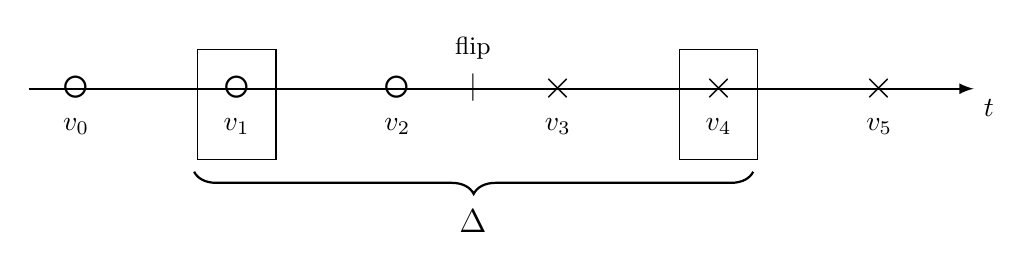
\begin{tikzpicture}[scale=1, line/.style={>=latex}] 

	\coordinate (t0) at (0, 0);
	\coordinate (t1) at (12, 0);

	\coordinate (b0) at (2.1, 0);
	\coordinate (b1) at (9.2, 0);

	\draw[->, line, color=black, thick]
		(t0) --
			node [pos=0.05, below=-8.5pt] {\huge $\circ$}
			node [pos=0.05, below=7pt] {$v_0$}
			node [pos=0.22, below=-8.5pt] {\huge $\circ$}
			node [pos=0.22, below=7pt] {$v_1$}
			node [pos=0.39, below=-8.5pt] {\huge $\circ$}
			node [pos=0.39, below=7pt] {$v_2$}
			node [pos=0.47, below=-9pt] {$ \mathbf{|} $}
			node [pos=0.47, above=7pt] {\small flip}
			node [pos=0.47, below=40pt] {\large $\Delta$}
			node [pos=0.56] {\Large $\times$}
			node [pos=0.56, below=7pt] {$v_3$}
			node [pos=0.73] {\Large $\times$}
			node [pos=0.73, below=7pt] {$v_4$}
			node [pos=0.90] {\Large $\times$}
			node [pos=0.90, below=7pt] {$v_5$}
			node [at end, below right] {$t$}
		(t1);

	\draw[draw=black] (2.14,0.5) rectangle ++ (1,-1.4);
	\draw[draw=black] (8.26,0.5) rectangle ++ (1,-1.4);
	
	\draw [
	    thick,
	    decoration={
		brace,
		amplitude=8pt,
		mirror,
		raise=30pt
	    },
	    decorate
	] (b0) -- (b1);

\end{tikzpicture}



	\caption{Illustration of a pMCI image pair, \Large$\circ$\normalsize\;= MCI, $\times$ = AD}
	\label{fig:pmci}
\end{figure}

Note that due to its use in the model validation, this data set represents a separate independent split, that is, subjects which are part of the MCI Conversion Set do not occur in any other split.

\subsubsection*{Leave One Visit Out} \label{sec:datloo}
Finally, as the name implies, the \textit{Leave One Visit Out Set} is formed by assigning one visit $v^s_i \in V(s)$ at random to the validation set for all subjects $s$ with $ | V(s) | \ge 3 $. All remaining visits are placed in the training set. Note that due to these criteria, this data set does not follow the global 5-fold split. See \autoref{tab:looset} for an overview of the data set.

\begin{table}[h]
	\begin{center}
		\begin{tabular}{c c c c c c c c c c c}
			\toprule
			\multirow{2}{*}{\bfseries Split} & 
			\multirow{2}{*}{\bfseries N} & 
			\multirow{2}{*}{\bfseries S} & 
			\multicolumn{2}{c}{\bfseries HC} & 
			\multicolumn{2}{c}{\bfseries MCI} & 
			\multicolumn{2}{c}{\bfseries AD} &
			\multicolumn{2}{c}{\bfseries Age} \\
			\cmidrule(lr){4-5}
			\cmidrule(lr){6-7}
			\cmidrule(lr){8-9}
			\cmidrule(lr){10-11} 
			& & & N & S & N & S & N & S & mean & std \\ 
			%------
			\cmidrule(lr){1-11}
			$\mathcal{S}_{train}$ & 16240 & 2794 & 5867 & 1338 & 6834 & 1164 & 3539 & 767 & 75.5 & 7.4 \\
			$\mathcal{S}_{valid}$ &  1599 & 1599 &  544 &  544 &  666 &  666 &  389 & 389 & 75.3 & 7.3 \\
			\cmidrule(lr){1-11}
			All                   & 17839 & 2794 & 6411 & 1343 & 7500 & 1183 & 3928 & 789 & 75.5 & 7.4 \\
			\bottomrule
		\end{tabular}
		\caption{Overview of the Leave One Visit Out data set. $N$ refers to the number of separate images and $S$ to the number of distinct subjects.}
		\label{tab:looset}
	\end{center}
\end{table}

\chapter{Experiments}

\section{Age Regressor} \label{sec:expagereg}
Validating the performance of a generative model is a hard problem in general. Beyond visual inspection of the outputs, we also pre-train an age regressor, which given an image $x$ produces an estimated age label $\hat a_x$, and use it to estimate the age label, and by extension the time step, of outputs generated by our model. Furthermore, the regressor is also included in the generator loss function as described in \autoref{sec:adaagereg}. Given its importance in the validation of our generative model, we evaluate the regressor's performance on a number of different tasks.

The regressor is implemented as a 3D CNN with nine layers, eight of which using batch normalization, and trained using the Adam optimizer with $\alpha = 0.001, \beta_1 = 0.9, \beta_2 = 0.999 $ and $ \epsilon = 0.0001 $.

\subsection*{Absolute Error}
First, we train the regressor for 30'000 batches of 32 samples each optimizing the absolute mean error as its objective function. Using our 5-fold data split, we perform cross validation and present the results in \autoref{tab:resagecrossval}. \autoref{fig:regxrxrhat} shows the estimated age $ \hat a_x $ against the ground truth label $a_x$ for one validation split. We note that the estimator tends to the mean, that is, its estimates are most accurate around the mean age across the data set of 75 years, and are low for subjects above the mean and high for subjects below the mean. Given the linear nature of the loss function, this is to be expected.

However, in our generative model, rather than estimating the absolute age of an image, the age regressor is used to estimate the relative age difference $a_y - a_x$ for an image pair $(x, y)$. Therefore, we further evaluate its performance on this task using our data set of image pairs. As before, we perform 5-fold cross validation and report the results in \autoref{tab:regagecrossval}. \autoref{fig:regxryr} compares the absolute losses for $x$ and $y$ and shows the error cancelling effect discussed in \autoref{sec:adaagereg}. Furthermore, we also estimate the age difference as $\hat a_y - \hat a_x$ for one split and visualize it against the ground truth time step in \autoref{fig:regddhatreal}. Using linear regression on our data points, we obtain an intercept of 0.03 and a slope of 0.67, indicating the estimated age difference tends to be too small for increasing $t$. This can be explained by closer examination of \autoref{fig:regxrxrhat} which shows that as the estimate $\hat a_x$ tends to the mean for labels futher away from it, relative age differences are subject to a shrinkage effect. 

Note that since we are performing these experiments on real image pairs, the results represent an upper bound for the performance of our generative model.
%TODO(crossval)

\begin{figure}
	\centering
	\includegraphics[width=.9\linewidth]{images/age_plots/xr_xrhat} 
	\vspace*{-15pt}
	\caption{Age regressor estimates on 2937 validation samples from our base image data set. Note how the predicitions tend to the mean, with a slope of 0.58 compared to the target of 1. The subject's diagnosis does not appear to have a major impact on the performance.}
	\label{fig:regxrxrhat}
\end{figure}

\begin{figure}
	\centering
	\includegraphics[width=.9\linewidth]{images/age_plots/xr_yr_dx} 
	\vspace*{-15pt}
	\caption{Age regressor estimates on 2651 validation samples from our pairs data set, with each axis representing one of the two images. While the absolute age error for a single image is quite significant with a mean of 3.39, the estimate of the relative age difference between two images from the same subject is considerably more accurate with a mean error of 1.21.}
	\label{fig:regxryr}
\end{figure}

\begin{figure}
	\centering
	\includegraphics[width=.7\linewidth]{images/age_plots/d_dhat_real}
	\vspace*{-15pt}
	\caption{Age regressor estimates on 2651 validation samples from our pairs data set, comparing the estimated age difference to the ground truth time step. Linear regression yields an intercept of 0.03 and a slope of 0.67. Note that the stripe patterns forming along the $x$-axis are a consequence of the study scheduling which mandates follow-up visits in intervals of six or twelve months.}
	\label{fig:regddhatreal}
\end{figure}

\subsection*{Squared Error}
We also examine the performance of the same architecture optimizing the mean squared error, with very similar if slightly inferior results presented in \autoref{tab:regagecrossval}

\subsection*{Leave One Visit Out}
Given that the age regressor is exclusively utilized to estimate relative age differences in our generative model, we perform an additional experiment more directly focussed at that metric. To that end, we train the same model architecture for 100'000 batches of 32 images each from the Leave One Visit Out data set outlined in \autoref{sec:datloo}. We obtain a mean absolute validation error of 1.01 TODO(exact) which, while significanlty lower than the mean absolute error on a single image, is still relatively large considering the simplified problem setting. However, the value is similar to the loss in the pair time step setting as expected. TODO(lame, maybe show that it doesn't simply overfit? Diff to other visits?)

\section{Diagnosis Classifier}
We pre-train a diagnosis classifier to discriminate between images labeled as MCI and AD respectively. Given the gradual transition between the two diagnoses, we use the \textit{MCI/AD Set} described in \autoref{sec:datmciad}, which limits our training and validation sets to a subset of images for which we have increased confidence in the diagnosis labels. Note that we exclude all subjects in the healthy control group HC and use a binary classifier focussing on the more subtle distinctions between the effects of MCI and AD. We train model is trained on TODO(number of batches) X batches of size 64, corresponding to Y TODO(number of epochs) epochs on our training set. We train all models a total of three times to avoid suboptimal local minima.

\section{Diffeomorphic Models}

\subsection{Voxelmorph}
To establish a baseline, we first train a variation of the Voxelmorph architecture described in \autoref{sec:vox} with minimal modifications to support the brain aging task. These modifications include removing the target image $y$ from the generator input as well as extending the scaling and squaring method to produce output deformations $\Phi^{(t)}$ for arbitrary $t$ as described in \autoref{sec:adaarbtimestep}. We report the results in TODO(what? Conversion? Visual inspection? Age plot?)

Note that we do not perform any hyperparameter tuning which might result in a significant improvement in performance.

\subsection{Synthetic Data}
To validate our modification to the architecture, we first train the model on 1'000 batches of 4 samples each from the synthetic data set described in \autoref{sec:synth}. The results, presented in \autoref{fig:toydata} and \autoref{tab:toydata} TODO(need this?), confirm the model's ability to learn and integrate over a stationary velocity field to generate deformation fields for variable time steps $t$. Furthermore, we demonstrate the effectiveness of the sparseness penalty in suppressing the deformation field in areas of little change. Note that neither the age regressor nor the diagnosis classifier are used in any of these experiments as there are no corresponding features in the synthetic data.

\begin{figure}
	\centering
	\usetikzlibrary{positioning}

\begin{tikzpicture}

	\coordinate (ref) at (0, 0);

	\node[below = 0.1 of ref] (nn) {\includegraphics[width=\textwidth]{images/toydata/no_noise_no_sparse}};

	\node[below = 0.1 of nn] (lnn) {no noise, no sparseness penalty};
	
	\node[below = 0.2 of lnn] (ny) {\includegraphics[width=\textwidth]{images/toydata/no_noise_sparse}};

	\node[below = 0.1 of ny] (lny) {no noise, with sparseness penalty};
	
	\node[below = 0.2 of lny] (yy) {\includegraphics[width=\textwidth]{images/toydata/noise_sparse}};

	\node[below = 0.1 of yy] (lyy) {noise, with sparseness penalty};

	\node[above right = 0.05 and 0.7 of nn.north west] (x) {$x\vphantom{\norm{v}_2}$};
	\node[right = 1.6 of x.west] (y)	{$y\vphantom{\norm{v}_2}$};
	\node[right = 1.6 of y.west] (yhat)	{$\hat y\vphantom{\norm{v}_2}$};
	\node[right = 0.9 of yhat.west] (t)	{$t\vphantom{\norm{v}_2}$};
	\node[right = 0.9 of t.west] (v)	{$v\vphantom{\norm{v}_2}$};
	\node[right = 1.4 of v.west] (mag)	{$\norm{v}_2$};
	\node[right = 1.8 of mag.west] (vx)	{$v_x\vphantom{\norm{v}_2}$};
	\node[right = 1.6 of vx.west] (vy)	{$v_y\vphantom{\norm{v}_2}$};
	\node[right = 1.6 of vy.west] (vz)	{$v_z\vphantom{\norm{v}_2}$};


\end{tikzpicture}

	\vspace*{-15pt}
	\caption{Model outputs generated using the synthetic data set. We train the model three times, on noisy or solid backgrounds, with or without applying a sparseness penalty. Each row represents one sample output consisting of the original, the target, and the generated image, the time step $t$ scaled to $[0, 1)$, the velocity field $v$ and its magnitude, as well as its separate dimensions. Note how the sparseness penalty leads to a more interpretable deformation field.} \label{fig:toydata}
\end{figure}

%TODO(NCC)

\subsection{MRI Data} %TODO(section title doesn't really make sense, more like adapted architecture, but then...)

\subsubsection*{Prediction}
%TODO(predict brain at real time step)
% with and without age regressor
% with training on s1-s4 vs. s1s3/s2s4
% discuss difference, reasons
Our first objective is to train the model to reproduce the time steps in our training data


\begin{figure}
	\centering
	\includegraphics[width=.7\linewidth]{images/age_plots/d_dhat_fake}
	\vspace*{-15pt}
	\caption{Age regressor estimates on 2651 validation samples $(x, \hat y)$ with $ \hat y = G(x) $ from our pairs data set, comparing the estimated age difference to the ground truth time step. Linear regression yields an intercept of 0.03 and a slope of 0.67. Note that the stripe patterns forming along the $x$-axis are a consequence of the study scheduling which mandates follow-up visits in intervals of six or twelve months.}
	\label{fig:regddhatfake}
\end{figure}

\begin{figure}
	\centering
	\includegraphics[width=\linewidth, trim={100 100 66 30}, clip]{images/HC_AD_plots/comp_ADNI_141445}
	\vspace*{-15pt}
	\caption{The center column contains a series of real images from a \textbf{subject diagnosed with Alzheimer's Disease}, taken at one-year intervals steps, top to bottom. The two columns to the left show the predicted images at the same time steps using a model trained exclusively on healty patients, as well as the difference maps with respect to the base image. Similarly, the two columns to the right show the predicted images using a model exclusively trained on patients affected by Alzheimer's Disease.}
	\label{fig:hcad_ad}
\end{figure}

\begin{figure}
	\centering
	\includegraphics[width=\linewidth, trim={100 100 66 30}, clip]{images/HC_AD_plots/comp_ADNI_137014}
	\vspace*{-15pt}
	\caption{The center column contains a series of real images from a \textbf{healthy subject}, taken at one-year intervals steps, top to bottom. The two columns to the left show the predicted images at the same time steps using a model trained exclusively on healty patients, as well as the difference maps with respect to the base image. Similarly, the two columns to the right show the predicted images using a model exclusively trained on patients affected by Alzheimer's Disease.}
	\label{fig:hcad_hc}
\end{figure}

\subsubsection*{Fixed Time Step Prediction}
%TODO(predict brain at fixed time step)
check resulting ages from age reg

\begin{figure}
	\centering
	\includegraphics[width=\linewidth]{images/age_plots/hist_fixed}
	\vspace*{-15pt}
	\caption{Age regressor estimates on 2651 validation samples from our pairs data set, comparing the estimated age difference to the ground truth time step. Linear regression yields an intercept of 0.03 and a slope of 0.67. Note that the stripe patterns forming along the $x$-axis are a consequence of the study scheduling which mandates follow-up visits in intervals of six or twelve months.}
	\label{fig:reghistfixed}
\end{figure}

\subsubsection*{Long-Term Prediction}
AD/HC only, compare
magnitude of flow differs (maybe numbers, but the finding is qualitative)
%TODO(mean flow plots)

% pat_id:	n_imgs	field		remark	base_img

% AD:
% ADNI_1066	7	1.5	pMCI	bad	ADNI_85356
% ADNI_922	7	1.5	pMCI		ADNI_77852
% ADNI_1427	7	1.5	pMCI 		ADNI_153734
% ADNI_42	8	1.5	pMCI	ugly
% ADNI_214	7	1.5	pMCI		ADNI_137475	maybe
% ADNI_906	6	1.5	pMCI	nice	ADNI_120065	yes, for now
% ADNI_887	6	1.5	pMCI		ADNI_120099	really nice, but need better model
% ADNI_658	6	1.5	pMCI		ADNI_62841	nope
% ADNI_752	6	1.5	pMCI		ADNI_66508	almost no changes
% ADNI_331	6	1.5	pMCI		ADNI_141445	yes! but better model
% ADNI_1243	6	1.5	pMCI	nice	ADNI_214258	small changes, okay

% HC:
% ADNI_382	8	1.5			ADNI_107542	okay...
% ADNI_441	8	1.5			ADNI_104027	nope
% ADNI_553	9	1.5			ADNI_155040	real kinda okay, AD model bad
% ADNI_677	8	1.5			ADNI_116851	no, messed up real
% ADNI_303	6	1.5		ugly	
% ADNI_337	10	1.5			ADNI_142666	no, artifacts
% ADNI_298	9	1.5			ADNI_141972	real okay, small ventricles, maybe slice 20, but guess not
% ADNI_734	8	1.5			ADNI_116000	yes, for now, not great though
% ADNI_120	10	1.5			ADNI_137014	good, slice 15
% ADNI_260	9	1.5			ADNI_172291	not really, skull, workable if need be

\subsubsection*{Conversion Prediction}
F1 score, accuracy

evalute our models ability to distinguish between stable and progressive cases of MCI

\chapter{Related Work}
Most similar to our work in terms of the problem setting, \cite{wegmayr} use a WGAN architecture to model the brain's aging process. They propose a UNet-derived model architecture based on \cite{baumgartner2018visual}, which is trained and applied iteratively to obtain predictions for different time steps. In addition to modeling the differences in the aging process between healthy subjects and subjects affected by Alzheimer's Disease, they report cautiously positive results for the task of conversion prediction.
\cite{baumgartner2018visual} use a WGAN on 3D MRI brain data to perform visual feature attribution and apply it to generate image-specific effect maps of Alzheimer's Disease.
In contrast to our work, the models used in \cite{wegmayr} and \cite{baumgartner2018visual} are entirely convolutional and do not use deformations.

Pursuing a similar goal, \cite{pathan2018predictive} use a combination of recursive and convolutional neural networks to predict a sequence of deformations based on, and then applied to, a baseline image to obtain follow-up predictions at different time steps. The model is trained on the first image of a subject as well as the sequence of diffeomorphic vector momenta for each additional image which are generated using the LDDMM framework \cite{beg2005computing}.

From a model perspective, the work most similar to ours is \cite{balakrishnan2019voxelmorph} \cite{dalca2018unsupervised}, which forms the basis of our work both in terms of the model design as well as its implementation. While the architecture was initially designed for unsupervised image registration, it has since been adapted to the problem of unsupervised segmentation \cite{dalca2019unsupervised}.
In the domain of face aging, \cite{palsson2018generative} suggest a conditional GAN \cite{mirza2014conditional} architecture similar to ours using an age regressor in the loss function.

As previously mentioned, early predictions of Alzheimer's Disease onset has been the target of considerable research efforts. \cite{thung2016identification} propose an SVM classifier distinguishing subjects with stable and progressive MCI and report an accuracy of 78.2\%. In contrast to our work, the features are extracted from longitudinal MRI brain data collected over a period of up to 18 months.
Reporting an accuracy of 92\%, \cite{sun2017detection} also use an SVM classifier on features extracted from a stationary velocity field, which is calculated using \cite{vercauteren2009diffeomorphic} on longitudinal data up to 36 months.

\chapter{Discussion}
Architecture with many components, hard to pinpoint problem origin

Interpretability of WGAN loss

Generative model output validation is hard, regressor as 
